\documentclass[technote]{IEEEtran}
\usepackage[top=1.5cm, bottom=1.4cm, left=1.6cm, right=1.6cm]{geometry}
\usepackage{graphicx}
\usepackage{amsmath}
\usepackage{amssymb}
\usepackage{braket}
\usepackage{cite}
\usepackage{tikz}
\usepackage[hidelinks]{hyperref}

\title{Quantum Memories via Microwave Electron Spin Ensembles}
\author{Linus Kelsey}

\begin{document}
\maketitle

\begin{abstract}
Quantum memories capable of faithfully storing and retrieving quantum states on demand are a critical enabling technology for quantum networks and distributed quantum computing. Electron spin ensembles in the solid state offer a compelling microwave-frequency platform: large ensembles facilitate strong coupling, while long intrinsic coherence times make spins natural registers. We review the physical basis and experimental progress in realising such memories, focusing on bismuth donors in silicon and three key advances: atomic clock transitions' use to push spin coherence beyond one second, the first quantum-level storage and retrieval of a superconducting qubit state in a spin ensemble, and a chirped pulse random-access protocol providing both spectral addressability and built-in dynamical decoupling. Remaining challenges, principally achieving unit spin-cavity cooperativity, are discussed alongside emerging directions including erbium-ion platforms that may ultimately bridge microwave memories to optical quantum networks.
\end{abstract}

\section{Introduction}

Fault-tolerant quantum computation at the application scale demands physical qubit counts that strain any foreseeable hardware architecture. Gidney and Eker{\aa} estimated that breaking RSA-2048 with Shor's algorithm requires approximately $2\times10^{7}$ physical qubits under the surface-code overhead typical of superconducting processors~\cite{gidney2021}, since revised below $10^6$~\cite{gidney2025}. Monolithic integration nonetheless remains impractical at this scale: Alexander notes that a 13-million-qubit superconducting chip would occupy a footprint of roughly $5\times5$\,m~\cite{alexander_thesis}. The quantum memory offers a compelling alternative, the quantum analogue of classical random access memory (RAM), offloading intermediate states from the processor, amortising qubit overhead across time. Gouzien and Sangouard show that RSA-2048 is broken with only 13,436 physical qubits when paired with a multimode quantum memory, three orders of magnitude fewer, requiring $\sim$\,1\,s multimode storage~\cite{gouzien2021}.

Realising this architecture imposes stringent constraints on the memory platform: superconducting qubits operate in the microwave regime (1-10\,GHz) at millikelvin temperatures, so any co-integrated memory must exchange microwave-frequency quantum states without requiring a frequency-conversion stage, itself introducing loss and noise. Electron spin ensembles in the solid state are a natural candidate, and modest spin densities can achieve strong coupling regimes inaccessible to single spins. These further benefit from the mature heritage of electron spin resonance (ESR) spectroscopy and, in carefully chosen host crystals, intrinsic coherence times extending to seconds.

This article reviews the physical basis and experimental progress of microwave spin-ensemble quantum memories, tracing the development from proof-of-concept through to the leading material platforms and two landmark experiments: the first quantum-level storage and retrieval of a superconducting qubit state, and a chirped-pulse random-access protocol. We close with discussion of remaining challenges and the emerging erbium transducer route to optical quantum networks.


\section{Spin Ensemble Platform}
\label{sec:platform}

The coupling of a spin ensemble to a single-mode microwave cavity is described by the Tavis-Cummings Hamiltonian, $H = \hbar\omega_c a^\dagger a + \sum_j \hbar\omega_j \hat{\sigma}_z^j/2 + \hbar g_0 \sum_j (a^\dagger \hat{\sigma}_-^j + a\hat{\sigma}_+^j)$, and under small excitations, the ensemble behaves as a bosonic mode with a collective coupling $g_\mathrm{eff} = g_0\sqrt{N}$. Even when $g_0/2\pi$ is only a few hertz, a spin density of order $10^{17}$\,cm$^{-3}$ in a sub-millimetre resonator mode volume is sufficient to enter the strong-coupling regime $g_\mathrm{eff} > \kappa, \gamma$, where $\kappa$ and $\gamma$ are the cavity and spin linewidths respectively - the central advantage for such a platform. For a broad review of spin systems relevant to this regime see Morton and Bertet~\cite{morton2018}.

Bismuth donors in silicon (Si:Bi) offer a rich hyperfine manifold from the $S = 1/2$ electron spin coupled to the $I = 9/2$ nuclear spin of $^{209}$Bi, generating ten ESR-accessible transitions in the microwave band. This manifold includes clock transitions at frequencies near 7\,GHz accessible at modest applied fields below 400\,mT, as characterised by O'Sullivan \textit{et al.}~\cite{O_sullivan_2020}. High-sensitivity single-spin readout of this system was previously demonstrated by Bienfait~\cite{Bienfait2016-zl}, providing the detection infrastructure on which memory experiments depend.

A fundamental limitation is inhomogeneous broadening: spatial variations in local crystal fields and strain distribute individual spin resonance frequencies across a bandwidth $\Delta\omega_\mathrm{inh}$ that typically exceeds $g_\mathrm{eff}$ by one to two orders of magnitude. The ensemble therefore dephases on a timescale $T_2^* \sim \Delta\omega_\mathrm{inh}^{-1}$ far shorter than the single-spin coherence time $T_2$. Recovering the stored state requires coherent refocusing, motivating both the clock-transition engineering described in Section~\ref{sec:coherence} and the pulse-based protocols of Section~\ref{sec:wurst}. Beyond Si:Bi, other spin systems have served as important demonstrations: nitrogen-vacancy centres in diamond were among the first to show ensemble coupling to a superconducting circuit~\cite{kubo2010}. Ytterbium-doped yttrium orthosilicate (Yb:YSO) is an emerging alternative, offering a zero-field clock transition (ZEFOZ) that sits naturally within the superconducting qubit operating band~\cite{alexander2022}.

\section{Coherence Engineering via Clock Transitions}
\label{sec:coherence}

Achieving long coherence in a solid-state spin ensemble requires suppression of three distinct decoherence channels: spectral diffusion from $^{29}$Si nuclear spin flip-flops producing a time-varying local field; instantaneous diffusion from dipolar coupling between simultaneously refocused spins; and direct donor--donor flip-flops at high doping concentrations. Together, these mechanisms constrain $T_2$ to the microsecond-to-millisecond range in most solid-state hosts.

Clock transitions, borrowed from precision atomic metrology, offer a means to suppress the dominant field-noise contribution - these are transitions insensitive to magnetic field fluctuations to first order. In the Si:Bi system the hyperfine structure gives rise to several such transitions at frequencies near 7\,GHz and applied fields below 400\,mT, placing them squarely within the operating band of superconducting quantum circuits. Wolfowicz \textit{et al.}\ exploited these transitions to extend the electron spin coherence time of $^{28}$Si:Bi to $T_2 = 2.7$\,s, representing a gain of several orders of magnitude over operation away from the clock point~\cite{wolfowicz2013}. At the clock transition, $^{29}$Si spectral diffusion is suppressed, leaving donor--donor flip-flops as the residual limit; even in natural silicon (4.7\% $^{29}$Si), $T_2 = 93$\,ms was achieved, greatly relaxing isotopic enrichment requirements.

On device integration, Wen \textit{et al.}\ recently demonstrated a tunable superconducting microresonator whose resonant frequency can be swept to match the clock transition of a Si:Bi ensemble~\cite{wen2025}, addressing a key practical obstacle: the clock-transition frequency is fixed by physics and the resonator must be brought to the spin, not the converse.


\section{Hybrid Architecture and Proof of Concept}
\label{sec:hybrid}

The canonical architecture for a spin-ensemble quantum memory integrates three components on a single chip: a superconducting qubit acting as the information source, a microwave bus resonator that mediates the coupling, and a spin ensemble serving as the storage register. State transfer proceeds by first swapping the qubit excitation into the bus, then tuning the bus into resonance with the spin ensemble to drive the excitation into the collective spin mode. This architecture was first realised by Kubo \textit{et al.}, who coupled a transmon qubit to an ensemble of nitrogen-vacancy centres in diamond through a frequency-tunable superconducting resonator acting as a quantum bus~\cite{kubo2011}. Arbitrary superpositions of the qubit state were written into collective excitations of the spin ensemble and later retrieved back into the qubit, constituting the first proof of concept of a spin-ensemble quantum memory for superconducting qubits. Ranjan \textit{et al.}\ demonstrated multimode microwave storage in bismuth donors in silicon using Hahn-echo refocusing - a $\pi$ pulse applied at half the storage time rephases the spin ensemble to recover a stored echo. The authors achieved storage times exceeding 100\,ms~\cite{ranjan2020}, the first demonstration of sub-GHz microwave quantum memory at the 100\,ms scale in any solid-state system, establishing the foundation for the random-access protocol described in Section~\ref{sec:wurst}.

\section{Random-Access Protocol}
\label{sec:wurst}

Hahn-echo storage suffers from two fundamental shortcomings that limit its utility as a quantum memory primitive. First, the $\pi$ refocusing pulse inverts the spin population, and amplified spontaneous emission from the resulting population inversion adds noise, fundamentally limiting retrieval fidelity, to the retrieved signal~\cite{ruggiero2009}. Second, multiple excitations stored by successive echo sequences are recalled in strict first-in-last-out order, precluding the random access essential for a quantum RAM architecture.

O'Sullivan \textit{et al.}\ resolved both using Wideband Uniform-Rate Smooth Truncation (WURST) pulses - chirped microwave pulses originally developed for broadband NMR refocusing~\cite{Kupce1995}. Each WURST $\pi$-pulse sweeps adiabatically through the inhomogeneous spin spectrum, inverting the ensemble dephasing trajectory ($k_\delta$, the net phase spread across spins; $k_\delta=0$ marks a rephased state where an echo can be emitted) and imprinting a chirp-parameter-dependent phase label~$\phi_W$. Varying the chirp rate or amplitude between pulse pairs produces distinct phase labels, giving each stored mode a unique address; the correct pair recalls only the intended mode while leaving others undisturbed. Matched pairs provide mode-selective storage and recall, as shown in Fig.~\ref{fig:wurst}. Repeated pairs additionally act as built-in dynamical decoupling, extending the memory lifetime to 2\,ms - a factor of three improvement over the Hahn-echo $T_2$.

\begin{figure}[t]
\centering
\scalebox{0.8}{%
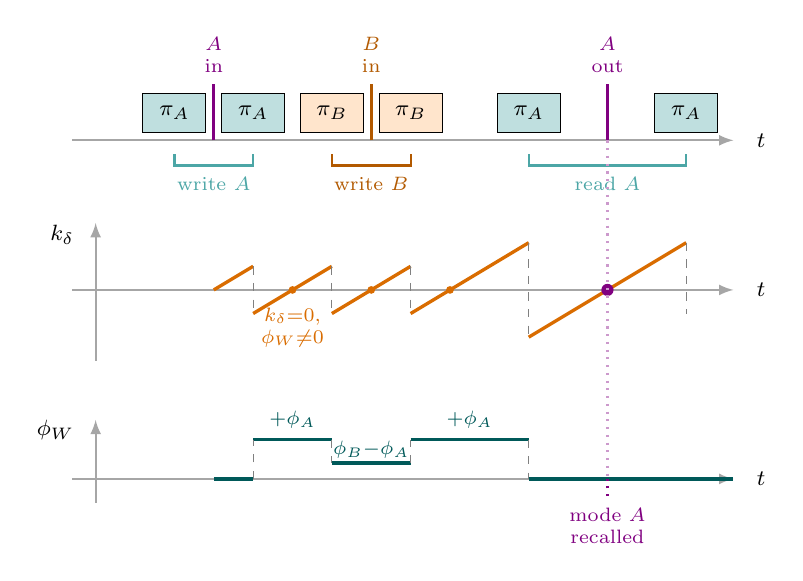
\begin{tikzpicture}[
  font=\footnotesize,
  wurst/.style={draw, fill=teal!25, minimum width=8mm, minimum height=5mm, inner sep=1pt},
  wurstB/.style={draw, fill=orange!20, minimum width=8mm, minimum height=5mm, inner sep=1pt},
  axline/.style={-latex, thick, gray!70},
]

% ---------- timing ----------
\def\T{8.1}
\def\tW{1.0}     % pi_A write 1
\def\tE{1.5}     % exc A absorbed
\def\tWb{2.0}    % pi_A write 2
\def\tB{3.0}     % pi_B 1
\def\tBe{3.5}    % exc B absorbed
\def\tBb{4.0}    % pi_B 2
\def\tR{5.5}     % pi_A read 1
\def\tEcho{6.5}  % echo A emitted
\def\tRb{7.5}    % pi_A read 2

% =====================================================
% ROW 1 : pulse sequence
% =====================================================
\begin{scope}[yshift=0cm]
  \draw[axline] (-0.3,0) -- (\T,0);
  \node at (\T+0.35,0) {$t$};

  % excitation A in
  \draw[very thick, violet] (\tE,0) -- (\tE,0.72);
  \node[violet, anchor=south, align=center, font=\scriptsize] at (\tE,0.74) {$A$\\in};

  % WURST pulses
  \node[wurst]  at (\tW, 0.35) {$\pi_A$};
  \node[wurst]  at (\tWb,0.35) {$\pi_A$};
  \node[wurstB] at (\tB, 0.35) {$\pi_B$};
  \node[wurstB] at (\tBb,0.35) {$\pi_B$};
  \node[wurst]  at (\tR, 0.35) {$\pi_A$};
  \node[wurst]  at (\tRb,0.35) {$\pi_A$};

  % excitation B in (between pi_B pair)
  \draw[very thick, orange!70!black] (\tBe,0) -- (\tBe,0.72);
  \node[orange!70!black, anchor=south, align=center, font=\scriptsize] at (\tBe,0.74) {$B$\\in};

  % echo A out (between read pi_A pair)
  \draw[very thick, violet] (\tEcho,0) -- (\tEcho,0.72);
  \node[violet, anchor=south, align=center, font=\scriptsize] at (\tEcho,0.74) {$A$\\out};

  % block brackets below axis
  \draw[teal!70, thick] (\tW,-0.18) -- (\tW,-0.32) -- (\tWb,-0.32) -- (\tWb,-0.18);
  \node[teal!70, font=\scriptsize, anchor=north] at ({(\tW+\tWb)/2},-0.34) {write $A$};

  \draw[orange!70!black, thick] (\tB,-0.18) -- (\tB,-0.32) -- (\tBb,-0.32) -- (\tBb,-0.18);
  \node[orange!70!black, font=\scriptsize, anchor=north] at ({(\tB+\tBb)/2},-0.34) {write $B$};

  \draw[teal!70, thick] (\tR,-0.18) -- (\tR,-0.32) -- (\tRb,-0.32) -- (\tRb,-0.18);
  \node[teal!70, font=\scriptsize, anchor=north] at ({(\tR+\tRb)/2},-0.34) {read $A$};
\end{scope}

% =====================================================
% ROW 2 : k_delta(t) for mode A, starting from tE
% rate = 0.6/unit; zero crossings at 2.5, 3.5, 4.5, 6.5(echo)
% =====================================================
\begin{scope}[yshift=-1.9cm]
  \draw[axline] (-0.3,0) -- (\T,0);
  \draw[-latex, thick, gray!70] (0,-0.9) -- (0,0.85);
  \node[anchor=east] at (-0.15,0.7) {$k_\delta$};
  \node at (\T+0.35,0) {$t$};

  \draw[very thick, orange!85!black]
    (\tE,0)     -- (\tWb,0.3)   % dephase: 0 to 0.3 in 0.5 units
    (\tWb,-0.3) -- (\tB,0.3)    % invert; zero at t=2.5, +0.3 at t=3.0
    (\tB,-0.3)  -- (\tBb,0.3)   % invert; zero at t=3.5, +0.3 at t=4.0
    (\tBb,-0.3) -- (\tR,0.6)    % invert; zero at t=4.5, +0.6 at t=5.5
    (\tR,-0.6)  -- (\tEcho,0)   % invert; zero at t=6.5 -> ECHO
    (\tEcho,0)  -- (\tRb,0.6);  % re-dephase; closed by second read pi_A

  % inversion jumps
  \draw[dashed, gray] (\tWb,0.3)  -- (\tWb,-0.3);
  \draw[dashed, gray] (\tB,0.3)   -- (\tB,-0.3);
  \draw[dashed, gray] (\tBb,0.3)  -- (\tBb,-0.3);
  \draw[dashed, gray] (\tR,0.6)   -- (\tR,-0.6);
  \draw[dashed, gray] (\tRb,0.6)  -- (\tRb,-0.3);

  % zero crossings: orange = suppressed, violet = echo
  \fill[orange!85!black] (2.5,0) circle (1.4pt);
  \fill[orange!85!black] (3.5,0) circle (1.4pt);
  \fill[orange!85!black] (4.5,0) circle (1.4pt);
  \fill[violet]          (\tEcho,0) circle (2.2pt);

  \node[orange!85!black, font=\scriptsize, anchor=north, align=center] at (2.5,-0.1)
    {$k_\delta{=}0$,\\\itshape $\phi_W{\neq}0$};
\end{scope}

% =====================================================
% ROW 3 : phi_W on mode A coherence
% 0 (tE-tWb), +phi_A (tWb-tB), phi_B-phi_A (tB-tBb), +phi_A (tBb-tR), 0 (tR+)
% =====================================================
\begin{scope}[yshift=-4.3cm]
  \draw[axline] (-0.3,0) -- (\T,0);
  \draw[-latex, thick, gray!70] (0,-0.3) -- (0,0.75);
  \node[anchor=east] at (-0.15,0.62) {$\phi_W$};
  \node at (\T+0.35,0) {$t$};

  \draw[very thick, teal!70!black]
    (\tE,0)    -- (\tWb,0)    % coherence dephasing; no WURST phase yet
    (\tWb,0.5) -- (\tB,0.5)  % +phi_A after write-2 pi_A
    (\tB,0.2)  -- (\tBb,0.2) % phi_B-phi_A after first pi_B
    (\tBb,0.5) -- (\tR,0.5)  % +phi_A restored: pi_B pair complete, A undisturbed
    (\tR,0)    -- (\T,0);    % phi_A cancelled by read-1 pi_A -> echo possible

  \draw[dashed, gray] (\tWb,0)   -- (\tWb,0.5);
  \draw[dashed, gray] (\tB,0.5)  -- (\tB,0.2);
  \draw[dashed, gray] (\tBb,0.2) -- (\tBb,0.5);
  \draw[dashed, gray] (\tR,0.5)  -- (\tR,0);

  \node[teal!70!black, font=\scriptsize, anchor=south] at ({(\tWb+\tB)/2},0.52) {$+\phi_A$};
  \node[teal!70!black, font=\scriptsize, anchor=north] at ({(\tB+\tBb)/2},0.6) {$\phi_B{-}\phi_A$};
  \node[teal!70!black, font=\scriptsize, anchor=south] at ({(\tBb+\tR)/2},0.52) {$+\phi_A$};

  % mode A recalled marker
  \draw[violet, thick, dotted] (\tEcho,-0.22) -- (\tEcho,0.05);
  \node[violet, font=\scriptsize, anchor=north, align=center] at (\tEcho,-0.24)
    {mode $A$\\recalled};
\end{scope}

% vertical guide at echo time
\draw[violet!40, dotted, thick] (\tEcho,0) -- (\tEcho,-4.3);

\end{tikzpicture}%
}% end scalebox
\caption{Random-access quantum memory with WURST chirped pulses. Each stored mode uses a matched WURST pair surrounding an excitation input (write), echo output (read), or null slot (dynamical decoupling). \emph{Write $A$}: excitation $A$ is absorbed between the two $\pi_A$ pulses; the second $\pi_A$ imprints $\phi_A$ on the coherence, suppressing the natural echo at the first $k_\delta{=}0$ crossing. \emph{Write $B$}: the matched $(\pi_B,\pi_B)$ pair stores excitation $B$ without disturbing mode $A$. \emph{Read $A$}: the first read $\pi_A$ cancels $\phi_A$; mode $A$ is emitted between the read pair when $k_\delta$ returns to zero. Mode $B$ remains stored, giving random access. After~\cite{osullivan2022}.}
\label{fig:wurst}
\vspace{-1.5ex}
\end{figure}

O'Sullivan \textit{et al.}\ demonstrated storage and retrieval of four independent excitations on demand in a bismuth-donor-in-silicon ensemble, with a spin-cavity cooperativity $C \approx 0.06$ and read-write efficiency of around 3\%~\cite{osullivan2022}. Approximately sixteen distinct WURST modes were resolved within the ensemble's inhomogeneous linewidth, and theoretical capacity reaches up to 100 modes alongside time-bin multiplexing.


\section{Challenges and Outlook}
\label{sec:outlook}

The dominant bottleneck across all demonstrated spin-ensemble memories is the spin-cavity cooperativity $C = g_\mathrm{eff}^2 / (\kappa\gamma)$. Storage efficiency scales as $4C/(1+C)^2$ in the impedance-matching limit~\cite{Afzelius_2013}, so $C = 1$ maximises the absorption of an incident field into the spin ensemble. The cooperativity achieved in the WURST demonstration thus explains the low efficiency. Reaching unit $C$ requires simultaneously maximising $g_\mathrm{eff}$ and the cavity quality factor $Q$. Actively investigated strategies include planar lumped-element microresonators that concentrate the microwave magnetic field $B_1$ into a smaller mode volume, increasing $g_0$~\cite{O_sullivan_2020}; isotopic enrichment of the silicon host to suppress the $^{29}$Si bath and extend spin coherence times, allowing higher active spin densities~\cite{wolfowicz2013}; and nuclear spin hyperpolarisation to pump the bismuth donor ensemble into a single nuclear spin state, raising the fraction of spins participating in the target ESR transition toward unity~\cite{morley2010}.

Si:Bi is fundamentally constrained by nuclear spin state occupancy: only the fraction of donors in the targeted hyperfine level contributes to $g_\mathrm{eff}$, capping cooperativity below unity without hyperpolarisation~\cite{O_sullivan_2020}. Yb:YSO closes this gap: Alexander \textit{et al.}\ coupled this system to planar NbN microresonators, reaching $C$ beyond the optimal point of unity ($C=4$--$245$) while preserving a ZEFOZ coherence time of 6\,ms, compatible out-of-the-box with superconducting qubits~\cite{alexander2022}. Hogan subsequently demonstrated operation of the WURST protocol at the efficiency-maximising $C=1$ threshold in Yb:YSO~\cite{hogan2026}; however, overall efficiency remained limited by losses elsewhere in the measurement chain. The critical importance of the cooperativity threshold for transfer efficiency was confirmed by Oehrl \textit{et al.}, who probed a phosphorus-donor spin ensemble in silicon at $C = 0.3$ using squeezed microwave states and directly observed the degraded transfer efficiency away from the $C = 1$ point~\cite{oehrl2025}. Addressing this gap between cooperativity and efficiency, Greggio \textit{et al.}\ have developed a theoretical framework for optimal time-dependent modulation of the cavity coupling during absorption and emission~\cite{greggio2026}, setting an efficiency benchmark for future experiments.

Beyond cooperativity and efficiency, erbium presents a route to bridging microwave spin memories to optical quantum networks. A spin system in its own right, Er$^{3+}$:CaWO$_4$ has exhibited coherence times of 23\,ms in natural-abundance CaWO$_4$ (no isotopic enrichment required) at millikelvin temperatures~\cite{dantec2021}. Erbium stands out for its optical transitions: individual ions in nanophotonic cavities have produced indistinguishable photons at 1532.6\,nm with spin coherence exceeding 200\,µs under dynamical decoupling~\cite{ourari2023}, and spin-photon entanglement has been demonstrated across 15.6\,km of standard optical fibre~\cite{uysal2024}. Together these establish three prerequisites for repeater nodes: coherence, indistinguishability, and fibre-compatible entanglement distribution. Rochman \textit{et al.}\ expanded on this, demonstrating simultaneous coupling of erbium ions to both a photonic resonator and a superconducting microwave resonator~\cite{rochman2023}, enabling microwave-to-optical conversion at the 1535\,nm telecom C-band. The long-term vision is a modular architecture in which a Yb:YSO or Si:Bi ensemble provides high-mode-count microwave storage local to the QPU, while an erbium transducer shuttles quantum information to fibre-optical networks - a capability that no individual spin species currently provides alone.


\section{Conclusion}

Electron spin ensembles in the solid state have, in the last fifteen years, evolved from proof-of-concept coupling demonstrations to a platform capable of second-scale coherence, random-access retrieval, and unit spin-cavity cooperativity. Storage times have exceeded 100\,ms, and spin-ensemble memories capable of storing hundreds of modes with near-unity efficiency are now a reasonable prospect. The combination of clock-transition coherence engineering in Si:Bi, which pushes $T_2$ beyond one second, with the WURST random-access protocol constitutes a viable architectural blueprint for a microwave RAQM. Erbium-based transduction offers a path toward connecting memories to optical quantum networks, enabling distributed quantum computing architectures. The achievement of $C = 1$ in Yb:YSO removes the last fundamental obstacle to high storage efficiency and shifts attention to engineering losses in the surrounding circuit. The primary remaining challenge is converting unit cooperativity into unit efficiency in a fully integrated device, a problem that now appears tractable given the theoretical guidance of optimal modulation protocols and the practical progress on planar microresonator design.


\bibliographystyle{IEEEtran}
\bibliography{references}

\end{document}
